\documentclass[11pt,fleqn, oneside,openany]{book} % Default font size and left-justified equations

% use this list: https://www.educative.io/blog/google-coding-interview

%%%%%%%%%%%%%%%%%%%%%%%%%%%%%%%%%%%%%%%%%%%%
%               Structure
%%%%%%%%%%%%%%%%%%%%%%%%%%%%%%%%%%%%%%%%%%%%
\input{sources/preamble.tex}

\interfootnotelinepenalty=10000

\begin{document}

%\frontmatter
%\begingroup
%\thispagestyle{empty}
%\begin{tikzpicture}[remember picture,overlay]
%  \coordinate [below=12cm] (midpoint) at (current page.north);
%  \node at (current page.north west)
%  {\begin{tikzpicture}[remember picture,overlay]
%      \node[anchor=north west,inner sep=0pt] at (0,0) {\includegraphics[width=\paperwidth]{images/background}}; % Background image
%\textsl{}
%      \draw[anchor=north] (midpoint) node [fill=ocre!30!white,fill opacity=0.6,text opacity=1,inner sep=1cm]{\Huge\centering\bfseries\sffamily\parbox[c][][t]{\paperwidth}{\centering Coding Interview Essentials\\[15pt] % Book title
%      {\Large - }\\[20pt] % Subtitle
%      {\huge Davide Spataro}}}; % Author name
%    \end{tikzpicture}};
%\end{tikzpicture}
%\vfill
%\endgroup


\includepdf[pages={2},fitpaper=true]{images/book_covers1.pdf}


\usechapterimagefalse % If you don't want to include a chapter image, use this to toggle images off - it can be enabled later with \usechapterimagetrue

%\chapterimage{images/header} % Table of contents heading image

\pagestyle{empty} % No headers

\tableofcontents % Print the table of contents itself

%\lstlistoflistings
%\listoffigures
%\listoftables

%\cleardoublepage % Forces the first chapter to start on an odd page so it's on the right

%pagestyle{fancy} % Print headers again

%!TEX root = ../main.tex
%%%%%%%%%%%%%%%%%%%%%%%%%%%%%%%%%%
% Links:
%
% Difficulty:
% Companies: 
%%%%%%%%%%%%%%%%%%%%%%%%%%%%%%%%%%


%\begin{figure}
%	\centering
%	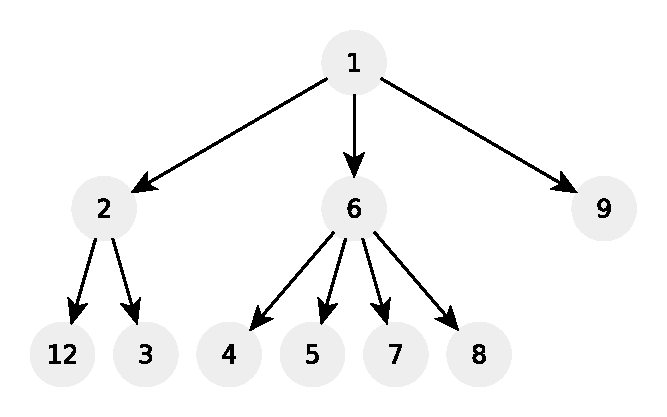
\includegraphics[width=\textwidth]{sources/coin_pickup/images/example1}
%	\caption[Sample short cpation]{Sample Caption}.
%	\label{fig:coin_pickup:example1}
%\end{figure}

\chapter{Coin Collection}
\label{ch:coin_pickup}
\section*{Introduction}

\section{Problem statement}
\begin{exercise}
\label{example:coin_pickup:exercice1}
You are given a square matrix $M$ of size $n \times n$ where each of its cells contains one of the following three integers:
\begin{enumerate}
	\item $0$: the cell is empty
	\item $1$: the cell contains a coin
	\item $-1$: the cell contains a thorn. 
\end{enumerate}

Write a function that returns the maximum number of coins you can collect by following the rules below:
\begin{itemize}
	\item You start at location $(0,0)$ (top-right corner) and you final goal is to reach the cell $(n-1,n-1)$ (bottom-left corner) by only moving down or right.
	\item From the cell $(n-1,n-1)$ you have to go back to the start location $(0,0)$, by only moving up or left.
	\item Cells containing $-1$ cannot be traversed.
	\item If you step into a cell containing a coin, you will automatically collect it.
\end{itemize}

	%example1
	\begin{example}
		\label{example:coin_pickup:example1}
		\hfill \\
		Given $M$  as in Figure \ref{fig:coin_pickup:example_1_0} the function return $4$.
		By starting from the top-left corner you can go twice down and twice right and reach the cell $(2,2)$. In the process
		you have collected $3$ coins (see highlighted cells in Figure \ref{fig:coin_pickup:example_1_1}).
		From cell $(2,2)$ you can then move left, then up twice and finally left to reach the starting cell $(0,0)$ again
		 and collecting the only coin left in cell $(0,1)$ (see the highlighted cells in Figure \ref{fig:coin_pickup:example_1_2}). 
	\end{example}

\end{exercise}

\section{Clarification Questions}


\begin{QandA}
	\item \begin{questionitem} \begin{question} Can a coin be collected twice if a cell with one in it is stepped into twice?  \end{question} 	 
    \begin{answered}
		\textit{No, once a cell with a coin is visited, it automatically becomes empty.}
	\end{answered} \end{questionitem}

	\item \begin{questionitem} \begin{question} What should the function return in case it is not possible to reach the botom-left corner of the matrix?   \end{question} 	 
		\begin{answered}
			\textit{If it is not possible to reach the cell $(n-1,n-1)$, the function should return $-1$.}
		\end{answered} \end{questionitem}
	

\end{QandA}


\begin{figure}
	\centering
	\begin{subfigure}[t]{0.3\textwidth}
		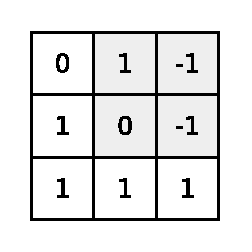
\includegraphics[width=1\linewidth]{sources/coin_pickup/images/example1_0}
		\caption{Input Matrix for the Example \ref{example:coin_pickup:example1}}
		\label{fig:coin_pickup:example_1_0}
	 \end{subfigure}
	\hfill
	\begin{subfigure}[t]{0.3\textwidth}
		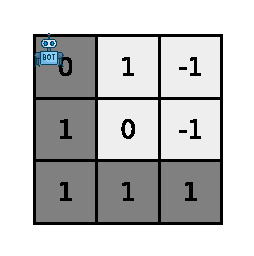
\includegraphics[width=1\linewidth]{sources/coin_pickup/images/example1_1}
		\caption{Path from $(0,0)$ to $(2,2)$ for an optimal solution to the Example \ref{example:coin_pickup:example1}.}
		\label{fig:coin_pickup:example_1_1}
	 \end{subfigure}
	 \hfill
	 \begin{subfigure}[t]{0.3\textwidth}
		 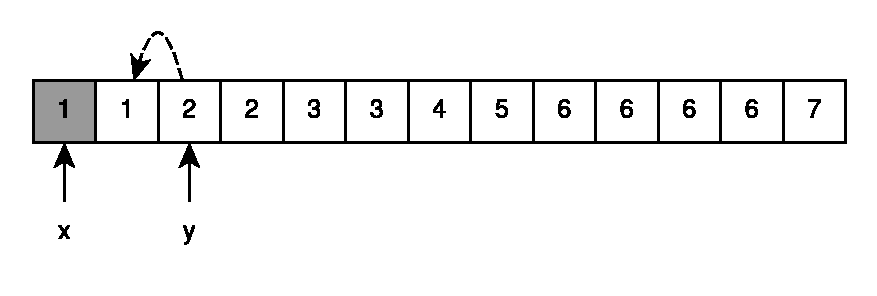
\includegraphics[width=1\linewidth]{sources/coin_pickup/images/example1_2}
		 \caption{Path from $(2,2)$ to the original starting location for an optimal solution to the Example \ref{example:coin_pickup:example1}.
		 Notice that the coins in the cells part of the path shown in Figure \ref{fig:coin_pickup:example_1_1} are collected.}
		 \label{fig:coin_pickup:example_1_2}
	  \end{subfigure}
\end{figure}


\section{Discussion}
\label{coin_pickup:sec:discussion}


\subsection{Brute-force}
\label{coin_pickup:sec:bruteforce}

\begin{minipage}{\linewidth}
	\lstinputlisting[language=c++, caption={Sample Caption},label=list:coin_pickup]{sources/coin_pickup/coin_pickup_solution1.cpp}
\end{minipage}



\section{Common Variations}
\subsection{Two robots}
A popular variation of the \textit{	\nameref{ch:coin_pickup}} problem is the one where
\begin{itemize}
	\item there are two robots navigating the matrix at the same time. 
	Robot $1$ starts from cell $(0,0)$ while robot $2$ starts from cell $(0,n-1)$.
	\item there are no constraints on the cells you have to reach meaning that you 
	do not have to go down to cell $(n-1,n-1)$ and then 
	\item each robot can move either down or down diagonally to the left and right and,
	\item the matrix is not necessarily square.
\end{itemize}.

\begin{exercise}
	\label{example:coin_pickup:variation1:exercice1}
	You are given a square matrix $M$ of size $n \times n$ where each of its cells contains an integer
	representing the number of coins in that cell. 
	
	There are two robots, $R1$ and $R2$, in the matrix, initially placed at locations: 
	\begin{enumerate*}
		\item $P_{R1}=(0,0)$
		\item $P_{R1}=(0,n-1)$
	\end{enumerate*}
	If a robot is at location $(x,y)$ in one step can move to cells: $(x+1,y)$, $(x+1,y-1)$ and $(x+1,y+1)$ as shown in Figure \ref{fig:coin_pickup:variation1:robot_movements}.
	Write a function returning the maximum number of coins you can collect with both $R1$ and $R2$.	
	
	
	\begin{example}
			\label{example:coin_pickup:variation1::example1}
			\hfill \\
			Given the input matrix is as the one shown in as in Figure \ref{fig:coin_pickup:variation1:example1} the function return $28$.
			$R1$ will collect all the coins along the path highlighted in green while $R2$ will collect the coins along the blue cells.
		\end{example}
	
\end{exercise}

\begin{figure}
	\centering
	\includegraphics[width=0.5\textwidth]{sources/coin_pickup/images/robot_movement_variation}
	\caption[Robot possible movements]{Robot movements pattern.}.
	\label{fig:coin_pickup:variation1:robot_movements}
\end{figure}



\begin{figure}
	\centering
	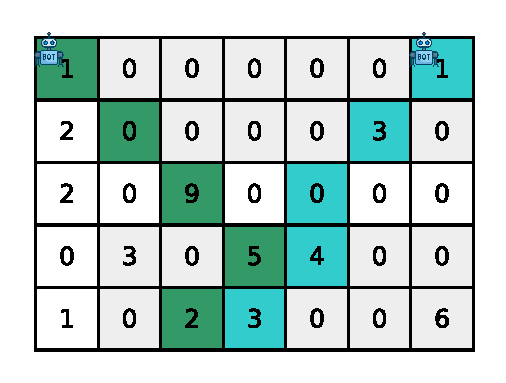
\includegraphics[width=0.9\textwidth]{sources/coin_pickup/images/variation1_example1}
	\caption[Robot possible movements]{Solution for the instance of the problem of the Example \ref{example:coin_pickup:variation1::example1}. Green and blue cell hightlight the paths of the first and second robot, respectively.}.
	\label{fig:coin_pickup:variation1:example1}
\end{figure}

%%%%%%%%%%%%%%%%%%%%%%%%%%%%%%%%%%%%%%%%%%%%
%               Appendices
%%%%%%%%%%%%%%%%%%%%%%%%%%%%%%%%%%%%%%%%%%%%

\chapter{Appendices}
%% @Author: Davide Spataro
% @Date:   2020-10-25 
% @Last Modified by:   Davide Spataro

\section{Dynamic Programming}
\label{sect:appendix:DP}

Dynamic programming (DP) is a popular tecnique for solving a certain class of
optimization problems efficiently and is accredited to the American Scientist
Richard Bellman\cite{bellman1954}. The word \textit{programming} can be a bit deceiving for
computer scientist of programmers in general but it has really little to do with
computer programming and it is infact intended as a set of rules to 
follow to solve a certain problem. These rules can of course be coded and
executed by a computer but can be easily followed on paper for instance. 
Dynamic programming is better thought as an optimization approach rather than an
method or framework where a complex optimization problem is transformed into a sequence of
smaller (and simpler) problems. The very essence of DP is its multi-stage
optimization procedure. DP does not provide directly with the
instruction on how to solve a particular problem, but instead provides a general
framework that requires creativity and non trivial effort/insights so that a
problem formulation can be adapted and casted within the DP framework bounds.
This is possibly the reason why DP is considered a rather hard topic and it is
particularly feared during interviews. 

This chapter is not intended to be a full treatement of DP, and we will
introduce and describe it to the level that is necessary to understand and
better tackle DP interview problems. For a more comprenshive material on DP
please refer to \cite{bellman1954, cormen2009}.


%\section{Prefix sum}
In computer science, the prefix sum, cumulative sum, inclusive scan, or simply scan of a sequence of numbers x0, x1, x2, ... is a second sequence of numbers y0, y1, y2, ..., the sums of prefixes (running totals) of the input sequence:
%% @Author: Davide Spataro
% @Date:   2020-03-30 17:18:14
% @Last Modified by:   Davide Spataro
% @Last Modified time: 2020-03-30 17:28:08
\section{Binary Search}
\label{sect:appendix:binary_search}
\lipsum{1}
%%%%%%%%%%%%%%%%%%%%%%%%%%%%%%%%%%%%%%%%%%%%
%               BIBLIOGRAPHY
%%%%%%%%%%%%%%%%%%%%%%%%%%%%%%%%%%%%%%%%%%%%

%
%from documentation
%\newacronym[⟨key-val list⟩]{⟨label ⟩}{⟨abbrv ⟩}{⟨long⟩}
%above is short version of this
% \newglossaryentry{⟨label ⟩}{type=\acronymtype,
% name={⟨abbrv ⟩},
% description={⟨long⟩},
% text={⟨abbrv ⟩},
% first={⟨long⟩ (⟨abbrv ⟩)},
% plural={⟨abbrv ⟩\glspluralsuffix},
% firstplural={⟨long⟩\glspluralsuffix\space (⟨abbrv ⟩\glspluralsuffix)},
% ⟨key-val list⟩}

\newacronym{cd}{CD}{compact disk}
\newacronym{utc}{UTC}{Coordinated Universal Time}
%\newacronym{adt}{ADT}{Atlantic Daylight Time}
%\newacronym{est}{EST}{Eastern Standard Time}
 
% Use the acronyms
\gls{utc} is 3 hours behind \gls{adt} and 10 hours ahead of \gls{est}.



%\addcontentsline{toc}{chapter}{\textcolor{ocre}{Glossary}}
%\printglossaries


%Print the glossary

\addcontentsline{toc}{chapter}{\textcolor{ocre}{Bibliography}}
%\chapter*{Bibliography}
%Print the glossary
\printbibliography	
	
%%%%%%%%%%%%%%%%%%%%%%%%%%%%%%%%%%%%%%%%%%%%
%               INDEX
%%%%%%%%%%%%%%%%%%%%%%%%%%%%%%%%%%%%%%%%%%%%	
	\cleardoublepage
	\phantomsection
	\setlength{\columnsep}{0.75cm}
	\addcontentsline{toc}{chapter}{\textcolor{ocre}{Index}}
	\printindex


	%\backmatter

\end{document}
